\chapter{Résumé long - conférence Mérigeo 2020} \label{merigeo}

\newpage
\newpage

\fontsize{14}{14}{\noindent\textbf{Photogrammétrie sous-marine et analyses d'images pour le suivi d'habitats benthiques Méditerranéens}}
\normalsize
\medskip

% Auteurs
\noindent MARRE Guilhem, DETER Julie, HOLON Florian, LUQUE Sandra
\medskip

% NB sans indentation
%\noindent\href{https://doi.org/10.3389/fmars.2019.00276}{\textit{Marre G, Holon F, Luque S, Boissery P and Deter J (2019) Monitoring Marine Habitats With Photogrammetry: A Cost-Effective, Accurate, Precise and High-Resolution Reconstruction Method. Front. Mar. Sci. 6:276. doi: 10.3389/fmars.2019.00276}}

%\medskip

\section*{Introduction}

Les pressions anthropiques et les changements globaux affectent la plupart des écosystèmes, et les écosystèmes marins ne font malheureusement pas exception à la règle. Le suivi de leur état de santé dans le temps nécessite de développer des méthodes d’observation permettant de contourner les contraintes physiques et physiologiques inhérentes au monde sous-marin. Parmi elles, la photogrammétrie permet, à partir d’une acquisition photographique relativement rapide en plongée, de reproduire en trois dimensions (3D) un habitat avec une grande précision. Ces modèles 3D peuvent être exploités pour réaliser une cartographie fine échelle et pour dériver un certain nombre de paramètres caractéristiques de l’objet d’étude et de leur évolution dans le temps. Par ailleurs, le développement récent d’algorithmes de reconnaissance d’image dits « d’apprentissage profond », conjointement à l’explosion des puissances de calculs et un accès toujours plus important à la donnée, permet aujourd’hui d’automatiser des tâches complexes comme la reconnaissance d’espèces sur des images sous-marines.

\medskip

\begin{tcolorbox}[colback=white,%gray background
                  colframe=black,% black frame colour
                  width=\linewidth,% Use 5cm total width,
                  arc=3mm, auto outer arc,
                 ]
Dans ce contexte, nous avons développé des méthodes basées sur de \textbf{l’analyse d’images} et la \textbf{photogrammétrie} pour le suivi des deux écosystèmes les plus riches de Méditerranée: les herbiers de Posidonie et les récifs coralligènes.
\end{tcolorbox}


\section*{Cartographie des herbiers de posidonie par photogrammétrie}

Les herbiers de Posidonie (\textit{Posidonia oceanica}) fournissent de précieux services écosystémiques (stockage carbone, nurserie à poissons, atténuation de houle…). Ils sont cependant soumis à d’importantes pressions anthropiques affectant directement les herbiers (mouillage) ou indirectement par la qualité de l’eau (turbidité, pollutions chimiques …). La qualité de l’eau, notamment sa capacité à transmettre la lumière naturelle, a des effets directs sur la limite inférieure des herbiers (limite profonde au-delà de laquelle on n’observe plus d’herbiers principalement à cause du manque de lumière). Il est donc primordial de suivre cette limite inférieure afin de rapidement diagnostiquer l’état d’un herbier (régression / progression) et avec du recul de déterminer les facteurs de cette évolution afin d’engager des décisions de gestion efficaces.


\subsection*{Méthodologie}
La méthode développée utilise le nuage de points éparse produit lors de la première étape de la chaîne de production des modèles par photogrammétrie (alignement des images dans l’espace 3D). Ce nuage de points contient l’ensemble des points d’appariement reconnus entre les différentes images du jeu de données. Mais la Posidonie possède une texture relativement homogène et n’est jamais parfaitement figée, y compris dans les conditions les plus calmes. De ce fait, peu de points d’appariement sont retenus dans l’herbier, et ceux qui le sont ont généralement une forte incertitude de reconstruction (cf Figure \ref{figureB.1}).

%%%%%%%%%%%%%%%%%%%%%%%%%%%%%%%%%%%%%%%%%%%%%%
%%% Figure B.1: Tâches d'herbier de Posidonie %%%
%%%%%%%%%%%%%%%%%%%%%%%%%%%%%%%%%%%%%%%%%%%%%%
\begin{figure}[htpb]
	\begin{center}
	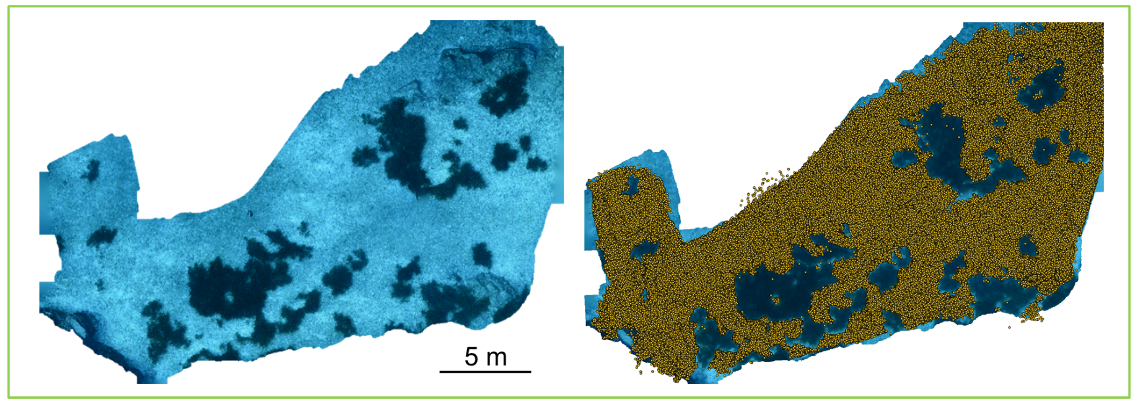
\includegraphics[width=\linewidth]{images/appendix_merigeo/Figure1.png}
		\caption[Tâches d’herbier de Posidonie visibles dans le nuage de points épars]{Tâches d’herbier de Posidonie visibles dans le nuage de points épars après alignement des images (Cappo Rosso, Corse, 2017)}
	\label{figureB.1}
\end{center}
\end{figure}

La méthode exploite cette propriété du nuage de points épars pour cartographier les herbiers: le nuage de points épars est filtré sur l’incertitude de reconstruction, converti en image binaire, soumis à des traitements morphologiques puis converti en polygones (cf Figure \ref{figureB.2}).

\newpage
\subsection*{Résultats}
%%%%%%%%%%%%%%%%%%%%%%%%%%%%%%%%%%%%%%%%%%%%%%
%%% Figure B.2: Résultats classification Posidonie %%%
%%%%%%%%%%%%%%%%%%%%%%%%%%%%%%%%%%%%%%%%%%%%%%
\begin{wrapfigure}[8]{R}{.5\textwidth} 
	%\begin{center}
	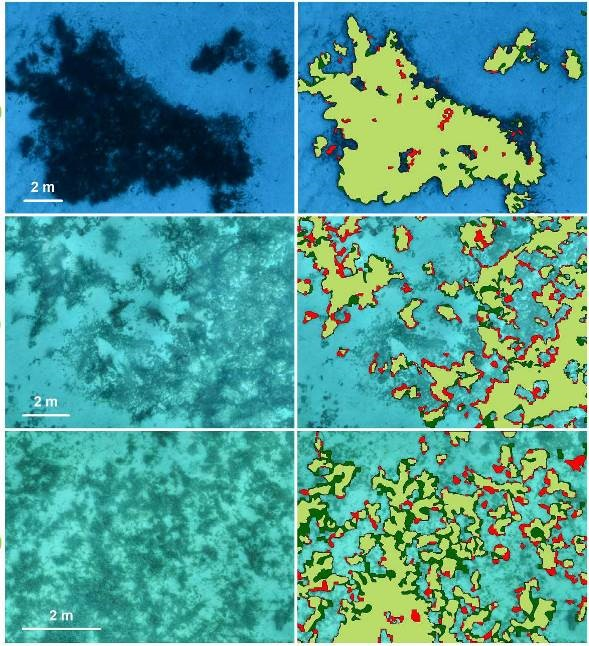
\includegraphics[width=7cm]{images/appendix_merigeo/Figure2.jpg}
		\caption[Résultats de classification pour trois niveaux de fragmentation différents]{Résultats de classification pour trois niveaux de fragmentation différents (en vert clair : les vrais positifs ; en rouge : les faux négatifs ; en vert foncé : les faux positifs)}
	\label{figureB.2}
%\end{center}
\end{wrapfigure}
Testée et optimisée sur 21 sites en limite inférieure, la méthode atteint un \textbf{F1 score moyen de 0.84}, pour une \textbf{précision} et un \textbf{taux de rappel moyens de 0.79 et 0.91}, respectivement. Si les performances sont indépendantes de la nature du substrat, de la profondeur et de la densité d’herbier, ils sont \textbf{affectés par le niveau de fragmentation} de l’herbier. 


\bigskip

\section*{Suivi de communautés coralligènes par des réseaux de neurones convolutifs}

Les récifs coralligènes sont situés entre 15 et 120 m de fond, et les communautés qui les composent sont d’une grande richesse (plus de 1500 espèces). La caractérisation des assemblages se fait classiquement par l’interprétation par un taxonomiste de quadrats photographiques pris en plongée (cf Figure \ref{figureB.3}. Forts d’une base de données de plus de 700 000 annotations sur plus de 10 000 quadrats depuis 2010 (réseau \acrshort{recor}), nous avons entraîné un réseau de neurones convolutif pour automatiser la reconnaissance d’espèces du coralligène.



%%%%%%%%%%%%%%%%%%%%%%%%%%%%%%%%%%%%%%%%%%%%%%
%%% Figure B.3: Quadrats photographique %%%
%%%%%%%%%%%%%%%%%%%%%%%%%%%%%%%%%%%%%%%%%%%%%%
\begin{figure}[htpb]
	\begin{center}
	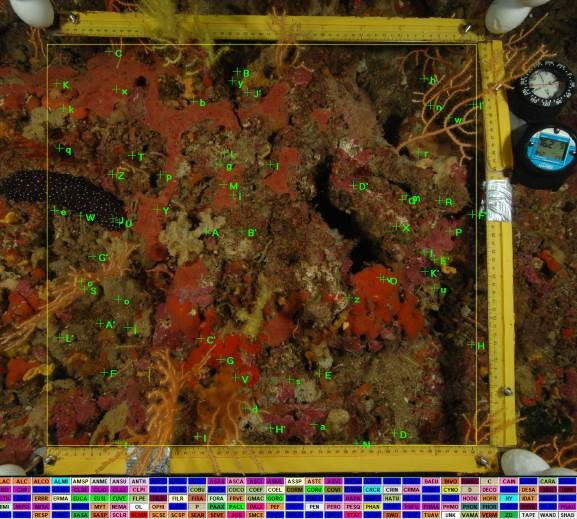
\includegraphics[width=8cm]{images/appendix_merigeo/Figure3.jpg}
		\caption[]{Quadrat photographique}
	\label{figureB.3}
\end{center}
\end{figure}


\subsection*{Méthodologie}
La base de données étant des annotations de points aléatoirement projetés sur des quadrats, nous avons entraîné un réseau de neurones de type ResNet18 sur des vignettes centrées sur ces pixels. Par ailleurs, les individus ou colonies pouvant prendre des tailles différentes d’une espèce à l’autre, nous avons entraîné quatre réseaux sur différentes tailles de vignettes (64, 69, 128 et 224 pixels), puis un réseau prenant en entrée les descripteurs appris par les quatre réseaux.

\subsection*{Résultats}

L’ensemble final de réseaux obtient un \textbf{F1 score de 0.72} pour la reconnaissance de \textbf{61 classes} d’organismes vivants et de substrat (qui représentent > 95 \% de notre base de données). Par ailleurs, un outil de \textbf{classification semi-automatique} permet de classer uniquement les vignettes pour lesquelles le taux de confiance est élevé, et laisser les autres à un taxonomiste expert. On obtient ainsi un \textbf{taux d’erreur de 20 \% pour 80 \% des images classées}.


En dégradant le niveau de détail à \textbf{15 classes}, le F1 score obtenu est de \textbf{0.84}. Ce score est \underline{supérieur à celui obtenu par plusieurs experts taxonomistes} sur un problème similaire sur 20 classes en milieu corallien. 


\section*{Suivi de la recolonisation d’un récif coralligène après restauration}
Suite à des travaux d’aménagements sur une conduite de rejet de station d’épuration en 2007, un récif coralligène a été enseveli sous des gravats à Saint Jean-Cap-Ferrat entre 35 et 45 m de fond. En collaboration avec la métropole Nice Côte d’Azur et l’Agence de l’Eau Rhône-Méditerranée-Corse, nous avons entrepris en septembre 2018 et avril 2019 des travaux de restauration écologique en excavant le récif enseveli depuis 10 ans. Depuis, nous suivons la recolonisation du récif par photogrammétrie tous les six mois.

\subsection*{Méthodologie}
Afin de suivre précisément l’évolution de la recolonisation, nous avons défini 14 quadrats permanents sur la surface nettoyée. Nous avons développé une méthode permettant, à partir des acquisitions 3D réalisées à chaque suivi, de produire un quadrat photographique avec exactement la même emprise spatiale. Il est ainsi possible de cartographier précisément l’état de surface et les espèces fixées à chaque pas de temps pour suivre les étapes de la recolonisation (cf Figure \ref{figureB.4}).


%%%%%%%%%%%%%%%%%%%%%%%%%%%%%%%%%%%%%%%%%%%%%%
%%% Figure B.4: Quadrat permanent %%%
%%%%%%%%%%%%%%%%%%%%%%%%%%%%%%%%%%%%%%%%%%%%%%
\begin{figure}[htpb]
	\begin{center}
	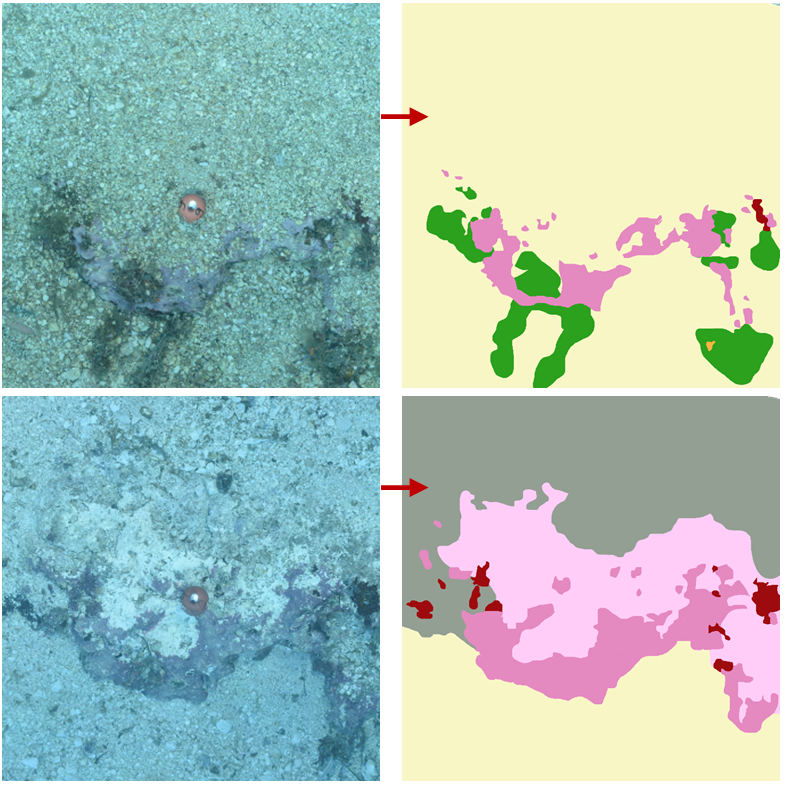
\includegraphics[width=10cm]{images/appendix_merigeo/Figure4.PNG}
		\caption[Quadrat permanent réalisé par photogrammétrie avant et après travaux de restauration]{Quadrat permanent réalisé par photogrammétrie avant et après travaux de restauration de septembre 2018 et analyses des communautés (Jaune = substrat meuble ; Gris = substrat rocheux ; Rose clair = coralligène nécrosé ; Rose foncé = Corallinales ; Rouge = Peyssoneliales ; Orange = bryozoaires ; Vert = autres algues).}
	\label{figureB.4}
\end{center}
\end{figure}

\subsection*{Résultats}
Le nettoyage a fait apparaître du \textbf{coralligène nécrosé sur 65 \%} (en moyenne) de la surface des quadrats restaurés. Un an après le nettoyage, les résultats des analyses montrent une \textbf{recolonisation progressive du récif excavé} par des algues rouges, des bryozoaires et des ascidies.
